\begin{figure*}[ht]
  \centering
  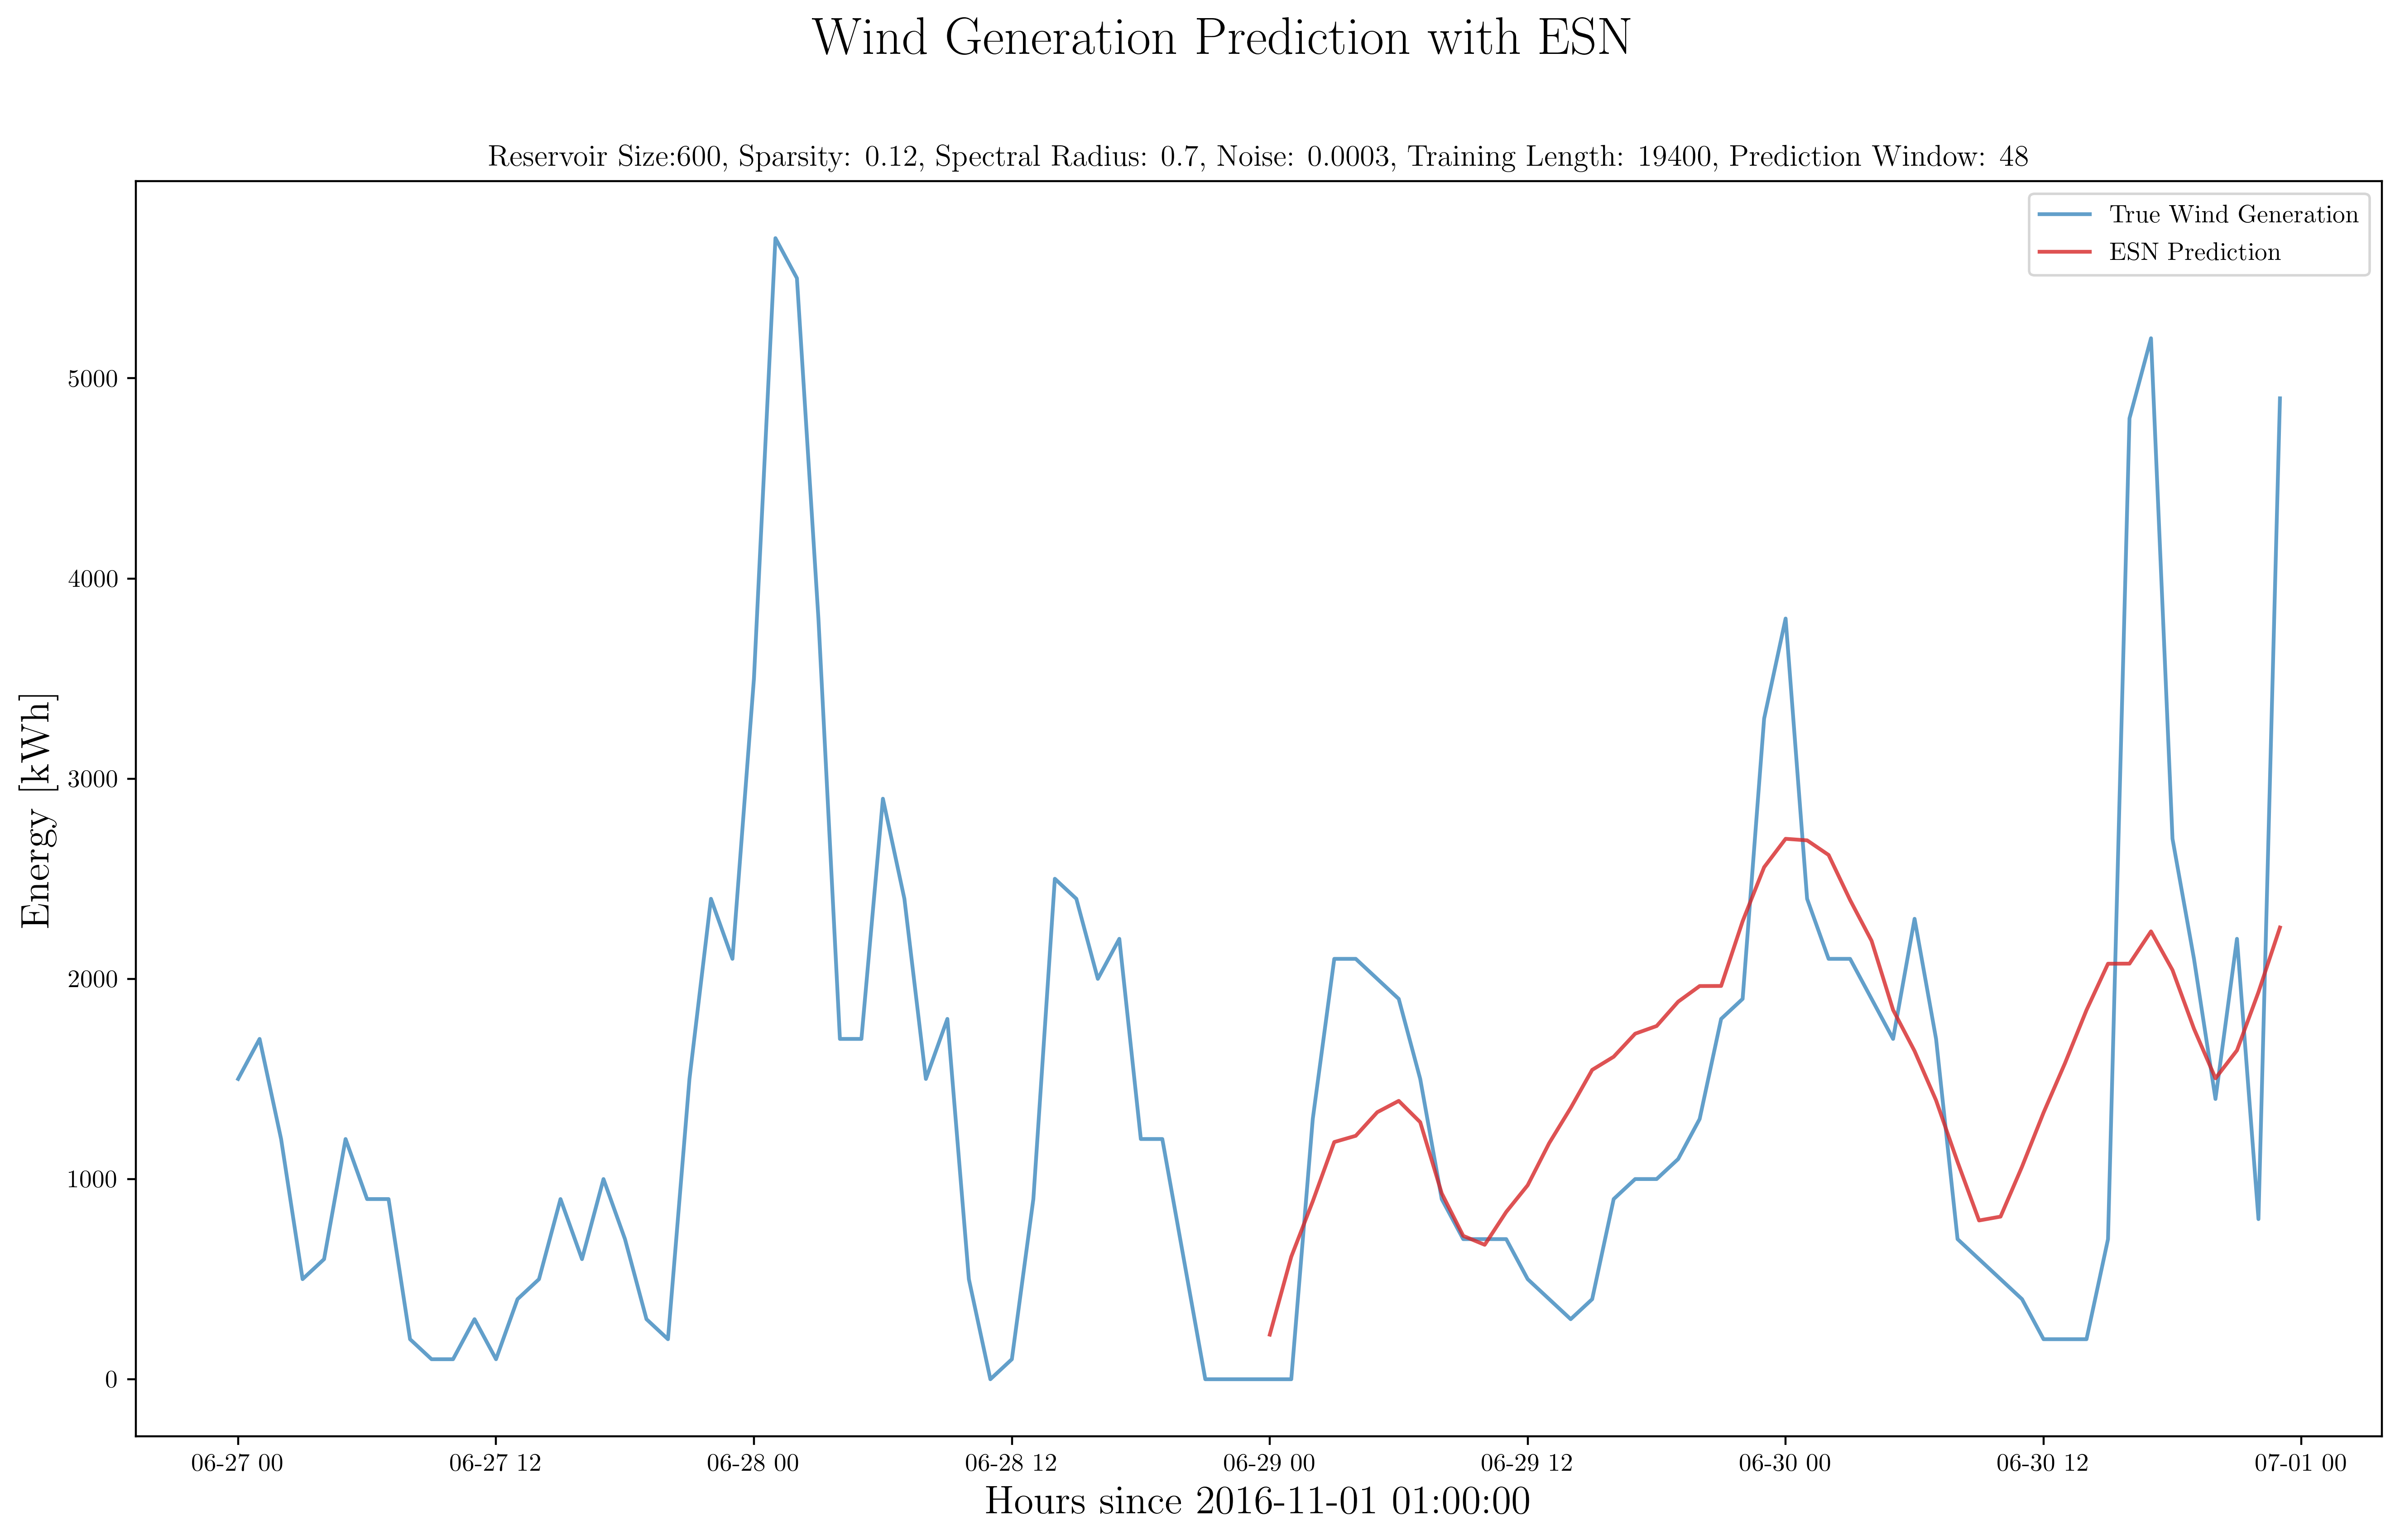
\includegraphics[width=0.8\textwidth]{48_wind_elevation_prediction.png}
  \caption{The optimized 48-hour ahead wind energy prediction with solar angle as an additional predictor.}
  \label{fig:wind48}
\end{figure*}
% \begin{center}
  \begin{table*}[ht]
    \centering
    \caption{Tabulated error for 48-hour ahead wind forecasts with various coupled quantities. Improvement indicates the percentage improvement over the base case of forecasting wind energy alone.}
    \label{tab:wind48}
    \begin{tabular}{l|c|c|c|c}
      &  & & l & Improvement \\
      Scenario  & MAE & RMSE & MAE (\%) & RMSE (\%)\\
      \hline
      Wind Energy & 0.103516 & 0.130848 & [-] & [-] \\
      Wind + Sun Elevation & 0.051899 & 0.081339 & -49.82 & -37.84\\
      Wind + Humidity & 0.091975 & 0.112054 & -11.15 & -14.36\\
      Wind + Pressure & 0.054388 & 0.097670 & -47.46 & -25.36\\
      Wind + Wet Bulb Temp. & 0.074085 & 0.097004 & -28.43 & -25.86\\
      Wind + Dry Bulb Temp. & 0.081268 & 0.105289 & -21.49 & -19.53\\
      Wind + Wind Speed & 0.100880 & 0.122271 & -2.5464 &-6.555 \\
    \end{tabular}
  \end{table*}
% \end{center}
